\documentclass[12pt, french]{article}
\usepackage{mhchem}
\usepackage{fancyhdr, fancybox, lastpage, makecell}
\usepackage[most]{tcolorbox}
\usepackage[a4paper, margin={0.3in, .75in}]{geometry}
\usepackage{wrapfig}
\pagestyle{fancy}
\renewcommand\headrulewidth{1pt}
\renewcommand\footrulewidth{1pt}
\fancyhf{}
\rhead{ \em{Zakaria Haouzan}}
\lhead[C]{\em{2ème année baccalauréat SM}}
\chead[C]{}
\rfoot[C]{}
\lfoot[R]{ \emph{ Transformation Spontanées dans les piles }}
\cfoot[]{\em{Page \thepage / \pageref{LastPage}}}


\newtcolorbox{Box2}[2][
enhanced,
breakable
]{
                lower separated=false,
                colback=white,
colframe=white!20!black,fonttitle=\bfseries,
colbacktitle=white!30!gray,
coltitle=black,
enhanced,
attach boxed title to top left={yshift=-0.1in,xshift=0.15in},
title=#2,#1}


\begin{document}
\begin{center}
   \shadowbox {\bf{Transformation Spontanées dans les piles et production d'énergie}}
\end{center}

\vspace{-0.2cm}
%%_________________________Exercice ! :"_________________________Exercice
%   \begin{center}
	   %\vspace{-0.6cm}
	%\includegraphics[width=0.6\textwidth ]{./img/Exercice01.png}
  %\end{center}
%\begin{wrapfigure}[2]{r}{0.48\textwidth}
  %\begin{center}
	  %\vspace{-1cm}
	%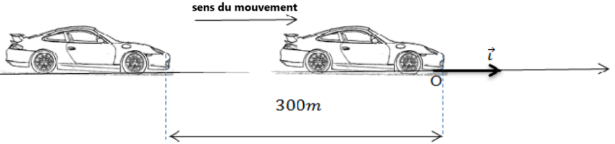
\includegraphics[width=0.48\textwidth]{./img/ex1.png}
  %\end{center}
%\end{wrapfigure}
%\begin{tcolorbox}\textbf{Exercice 2 : propagation d’ondes ultrasonores et des ondes lumineuses }
%\end{tcolorbox}





\begin{Box2}{\textbf{Exercice 1 : Étude de la pile plomb–étain}}
\begin{wrapfigure}[8]{r}{0.48\textwidth}
  \begin{center}
	  \vspace{-2cm}
	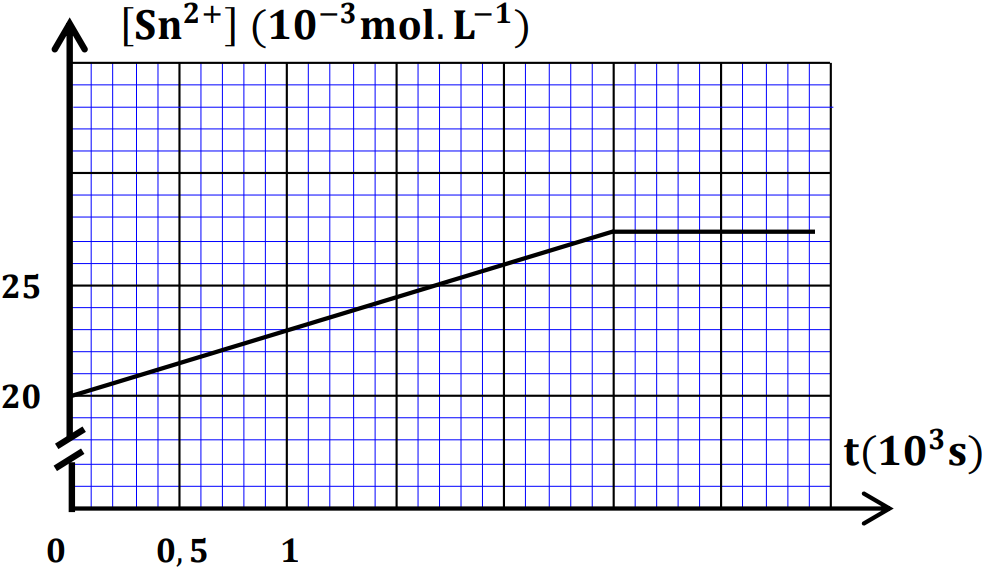
\includegraphics[width=0.48\textwidth]{./fig00P.png}
  \end{center}
\end{wrapfigure}
Les piles électrochimiques sont l'une des applications des réactions d'oxydo-réduction. Au cours de leur fonctionnement, une partie de l'énergie chimique se transforme en énergie électrique.

  On réalise, à $25^{\circ}$, la pile plomb–étain en plongeant une plaque de plomb dans un bécher contenant un volume $V_1 = 30 mL$ d’une solution aqueuse de nitrate de plomb $\text{Pb}^{2+} + 2\text{NO}_3^-$ de concentration molaire initiale $C_1^{0} = [\text{Pb}^{2+}]$, et en plongeant une plaque d’étain dans un autre bécher contenant un volume $V_2 = V_1$ d’une solution aqueuse de chlorure d’étain II $\text{Sn}^{2+} + 2\text{Cl}^-$ de concentration molaire initiale $C_2^{0} = [\text{Sn}^{2+}]$. Les deux solutions sont reliées par un pont salin contenant une solution saturée de chlorure d’ammonium $\text{NH}_4^+ + \text{Cl}^-$. 

On monte en série entre les pôles de la pile un conducteur ohmique (D), un ampèremètre et un interrupteur. On ferme l’interrupteur à l’instant $t=0$, un courant d’intensité $I = 17.13mA$ circule alors dans le circuit. La courbe ci-contre représente l’évolution temporelle de la concentration des ions $\text{Sn}^{2+}$.

\subsection*{Donnée} 
\begin{itemize}
  \item La constante de Faraday: $F=9,65.10^{4}C.mol^{-1}$.
\end{itemize}

  Soit $K$ la constante d’équilibre, à $25^{\circ}$, associée à l’équation de la réaction:

\begin{equation}
    \text{Pb}(s) + \text{Sn}^{2+}(aq) \rightleftharpoons \text{Sn}(s) + \text{Pb}^{2+}(aq)
\end{equation}

\subsection*{Questions} 
\begin{enumerate}
    \item En exploitant la courbe, déterminer le sens d’évolution du système chimique. (0,5pt)
    \item Écrire l’équation de la réaction qui se produit au niveau de l’anode. (0,25pt)
    \item Représenter le schéma conventionnel de la pile étudiée. (0,25pt)
    \item Déterminer le sens de migration des ions chlorure $\text{Cl}^-$ lors du fonctionnement de cette pile. (0,25pt)
    \item En utilisant le tableau d’avancement de la réaction:
    \begin{enumerate}
        \item Trouver, au cours du fonctionnement de la pile, l’expression de $[\text{Sn}^{2+}]$ à un instant $t$ en fonction de $V_2$, $C_2$, $F$, $I$ et $t$. (0,75pt)
        \item Montrer que:
        \begin{equation}
            K = \frac{2FC_2V_2 - I \Delta t}{2FC_2V_2 + I \Delta t}
        \end{equation}
        où $\Delta t$ est la durée maximale de fonctionnement de la pile. Calculer $K$. (1pt)
    \end{enumerate}
\end{enumerate}

\end{Box2}

%\vspace{1.6cm}

\begin{Box2}{Exercice 2 :Etude de la pile Cadmium – Argent }

On étudie la pile Cadmium – Argent qui fait intervenir les deux couples ox/red : $\text{Ag}^+/\text{Ag}$ et $\text{Cd}^{2+}/\text{Cd}$.

\subsection*{Données} 
\begin{itemize}
  \item Le Faraday : $F = 9,65.10^{4}{C.mol^{-1}}$.
    \item La constante d’équilibre associée à la réaction :
    \begin{equation}
        2\text{Ag}^+(aq) + \text{Cd}(s) \rightleftharpoons 2\text{Ag}(s) + \text{Cd}^{2+}(aq)
    \end{equation}
    $K = 5 \times 10^{40}$ à ${25^{\circ}}$.
    \item La masse molaire du Cadmium : $M(\text{Cd}) = {112.4}{g.mol^{-1}}$.
\end{itemize}

On réalise cette pile en plongeant une lame d’argent dans un bécher contenant un volume $V = {250}{mL}$ d’une solution aqueuse de nitrate d’argent $\text{Ag}^+ + \text{NO}_3^-$ de concentration molaire initiale $C_1^i = {0.400}{mol.L^{-1}}$, et une lame de cadmium dans un autre bécher contenant un volume $V = {250}{mL}$ d’une solution aqueuse de nitrate de cadmium $\text{Cd}^{2+} + 2\text{NO}_3^-$ de concentration molaire initiale $C_2^i = {0.200}{mol.L^{-1}}$. On relie ensuite les deux solutions par un pont salin.

On branche entre les électrodes de la pile un conducteur ohmique monté en série avec un ampèremètre et un interrupteur.

\begin{enumerate}
    \item Choisir la proposition juste parmi les affirmations suivantes :
    \begin{enumerate}
        \item Le pôle positif de la pile est l’électrode d’argent.
        \item L’oxydation se produit au niveau de la cathode.
    \end{enumerate}
    \item Exprimer, à un instant $t$, le quotient de réaction $Q_r$ en fonction de l’avancement $x$ de la réaction.
    \item Calculer $Q_r$ à l’instant $t = 10h$.
    \item Calculer la variation de la masse de l’électrode de cadmium entre l’instant $t=0$ et l’instant où la pile est usée.
\end{enumerate}

\end{Box2}

\end{document}
